\documentclass[12pt]{report}
\usepackage{graphicx}
\usepackage{subfig}
\usepackage{listings}
\usepackage{hyperref}

\begin{document}
\lstset{language=Python}

\title{Homework 1 - Applied Machine Learning}
\author{Tim Delisle and Sam Raudabaugh}
\date{09/15/2015}
\maketitle

\noindent{{\large 1a). Importing data files}}

In order to import our dataset we use the pandas library which creates a DataFrame object making accessing and parsing data a breeze. We also use matplotlib to display images, histograms and plots

http://pandas.pydata.org/

http://matplotlib.org/

\noindent{{\large 1b). Displaying a digits }}

In order to display a digit we split the digits using a pandas query for the appropriate label then we simply pick the first of each of these digit buckets to display. We then use the matplotlib function imshow to generate the images. See figure one for results. Our show digit function takes as input a digit gray scale values and outputs an image.
\begin{figure}
\centering
\subfloat[zero]{
  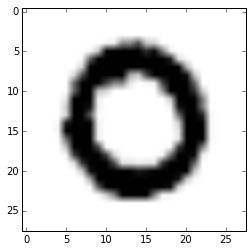
\includegraphics[width=25mm]{figures/zero.png}
}
\subfloat[one]{
  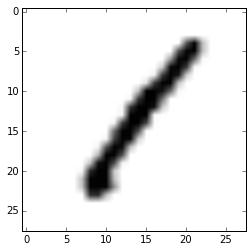
\includegraphics[width=25mm]{figures/one.png}
}
\subfloat[two]{
  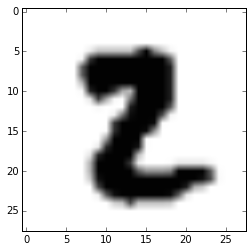
\includegraphics[width=25mm]{figures/two.png}
}
\subfloat[three]{
  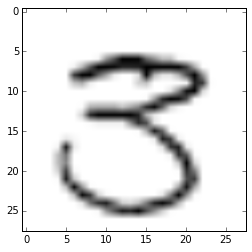
\includegraphics[width=25mm]{figures/three.png}
}
\subfloat[four]{
  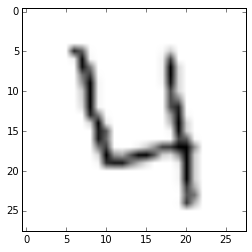
\includegraphics[width=25mm]{figures/four.png}
}

\subfloat[five]{
  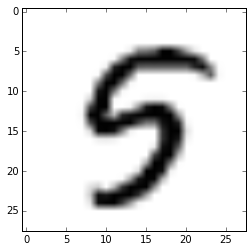
\includegraphics[width=25mm]{figures/five.png}
}
\subfloat[six]{
  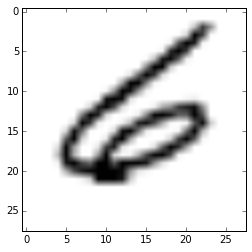
\includegraphics[width=25mm]{figures/six.png}
}
\subfloat[seven]{
  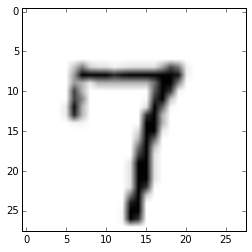
\includegraphics[width=25mm]{figures/seven.png}
}
\subfloat[eight]{
  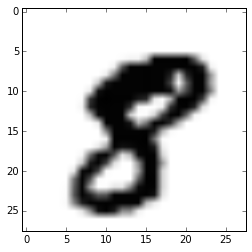
\includegraphics[width=25mm]{figures/eight.png}
}
\subfloat[nine]{
  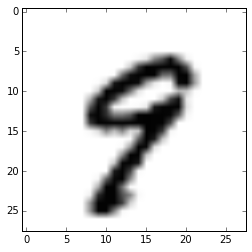
\includegraphics[width=25mm]{figures/nine.png}
}
\caption{Displaying each digit}
\end{figure}

\noindent{{\large 1c). Examining distribution of digits}}

We then plotted (using matplotlib's hist) the histogram of counts of each digit and saw a uniform distribution but not an equal number of each digit. See figure two.

\begin{figure}
\centering
\subfloat[]{
  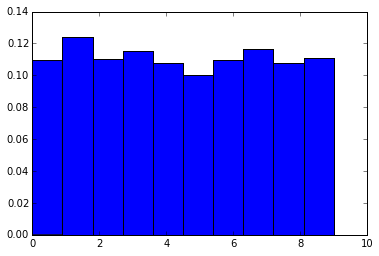
\includegraphics[width=50mm]{figures/digit_distribution.png}
}
\caption{Displaying each digit}
\end{figure}


\noindent{{\large 1d). Computing Nearest Neighbors for individual digits}}

We computed the nearest neighbor of the displayed digits above. The only mismatch was the 3 which was interpreted as a five. See output in figure 3. In this case we used the numpy linalg norm function to compute the euclidean distances.

\begin{figure}
\centering
\subfloat[]{
  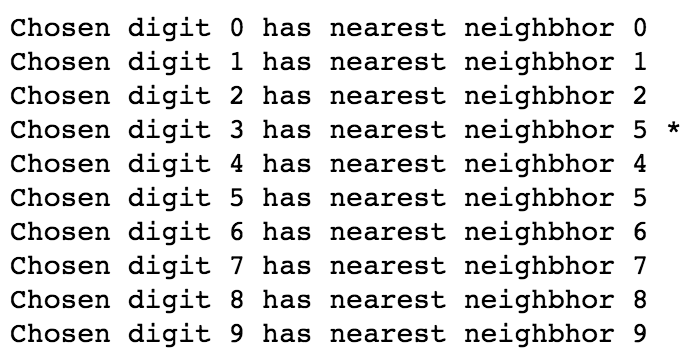
\includegraphics[width=50mm]{figures/single_digitNN.png}
}
\caption{Displaying each digit}
\end{figure}

\noindent{{\large 1e). Computing pairwise distances for 0s and 1s}}

For this part of the exercise we decided to parallelize the code in order to reduce the computation time. To do so we used iPython Parallel

http://ipython.org/ipython-doc/dev/parallel/

To parallelize the process we defined four engines, isolated zeros and ones from the original data and subsequently sent the data to each of the engines. 

Once the data is on each engine we compute the pairwise distances for each 0 vs 0s, 1 vs 1s and 0 vs 1s by simply looping through each of possible pair of digits and computing the euclidean distance. 

Once the distance matrices are computed we gather them from each engine and concatenate the matrices back into a single matrix for each genuine 0 vs 0, 1 vs 1 and 0 vs 1.

For all distance computations we get without dupliactes 1 loops, best of 3: 1min 45s per loop 4Cores

For gathering the data we get 1 loops, best of 3: 1min 17s per loop

For a total of 3min 02s .

We then plot the histograms for the genuine and importer pairs for zeros and ones.

\begin{figure}
\centering
\subfloat[Genuine vs Imposters ones]{
  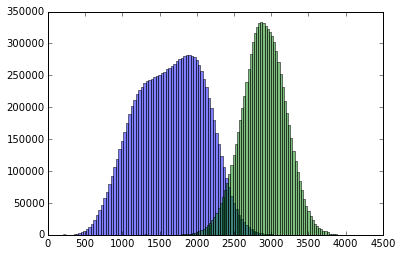
\includegraphics[width=75mm]{figures/hist_ones.png}
}
\subfloat[Genuine vs Imposters zeros]{
  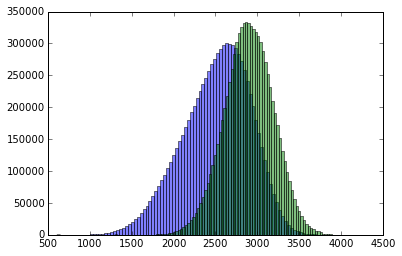
\includegraphics[width=75mm]{figures/hist_zeros.png}
}
\caption{Ones in histogram a and zeros in histogram b}
\end{figure}

\noindent{{\large 1f). Generating ROC curves for ones and zeros}}

We created ROC curves  by calculating the TPR and FPR rates by iteration. We stepped through the threshold values with step size = 10. We have equal error rates of ~.05 and ~.4 for ones and zeros respectively read from the graph. See ROC curve in figure 5.

\begin{figure}
\centering
\subfloat[ROC ones]{
  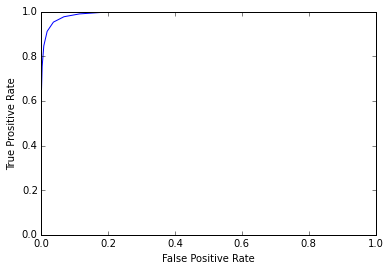
\includegraphics[width=75mm]{figures/ROC_ones.png}
}
\subfloat[ROC zeros]{
  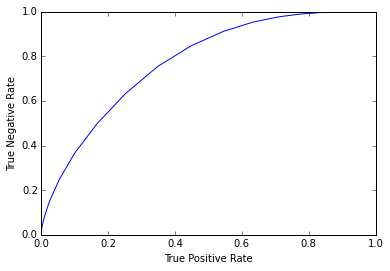
\includegraphics[width=75mm]{figures/ROC_zeros.png}
}
\caption{Ones in histogram a and zeros in histogram b}
\end{figure}

\noindent{{\large 1g). Implementing a KN-Neighbor}}

In our implementation of nearest neighbor we compute all the distances between two datasets, find the k-nearest of the distances and then find the majority vote class for the smallest distances. We use the following libraries to ensure that the run time is reasonable.

scipy

We use scipy's cdist function to compute all the euclidean distances between two matrices. This implementation is incredibly speedy drastically reducing the time to compute our predictions.

cdist: http://docs.scipy.org/doc/scipy/reference/generated/scipy.spatial.distance.cdist.html

numpy

We use numpy's ND array to facilitate matrix/vector operations which are implemented incredibly efficiently in this library. We also use numpy's argsort which finds the index of the minimums of a vector

Argsort: http://docs.scipy.org/doc/numpy/reference/generated/numpy.argsort.html

When determining the class winner for the n nearest neighbors we simply implement date minimum mode as the tie breaker. This is only pseudo random and therefore could be improved with a random mode picker if there are two modes of class in the n-nearest neighbors.


\noindent{{\large 1h and i). 3-fold + confusion matrices}}

In our implementation of 3-fold cross validation we split our dataset into three folds, then compute knn on 1, 2+3 | 2, 1+3 | 3, 1+2. We then generate a truth comparison of the label and the predicted value and  put these comparisons in a confusion matrix. We have the confusion matrices in the following table. We can see that fold one and three are of similar accuracy though something seems clearly wrong with fold two since its accuracy is significantly lower. For each fold the average accuracy is 96.7\%, 70.95\% and 96.7\% for folds one, two and three respectively. When using the entire train data as the test we get a 98\% average accuracy.

\begin{centering}
\begin{table}[h!]
\begin{tabular}{lllllllllll}

 & 0 & 1 & 2 & 3 & 4 & 5 & 6 & 7 & 8 & 9 \\
0 & 1359 & 1 & 2 & 0 & 0 & 2 & 6 & 1 & 0 & 0 \\
1 & 0 & 1566 & 2 & 2 & 0 & 0 & 2 & 0 & 1 & 2 \\
2 & 10 & 25 & 1353 & 5 & 2 & 1 & 0 & 25 & 4 & 2 \\
3 & 1 & 4 & 7 & 1369 & 0 & 15 & 0 & 5 & 6 & 3 \\
4 & 0 & 17 & 0 & 0 & 1313 & 0 & 5 & 3 & 0 & 30 \\
5 & 3 & 3 & 2 & 25 & 0 & 1217 & 14 & 1 & 3 & 8 \\
6 & 9 & 2 & 0 & 0 & 2 & 3 & 1383 & 0 & 0 & 0 \\
7 & 1 & 26 & 3 & 0 & 5 & 0 & 0 & 1412 & 0 & 17 \\
8 & 8 & 11 & 7 & 28 & 4 & 31 & 9 & 6 & 1223 & 16 \\
9 & 4 & 3 & 0 & 8 & 13 & 3 & 1 & 23 & 3 & 1309 \\

\end{tabular}
\caption{Fold one confusion matrix}
\end{table}

\begin{table}[h!]
\begin{tabular}{lllllllllll}

 & 0 & 1 & 2 & 3 & 4 & 5 & 6 & 7 & 8 & 9 \\
0 & 1179 & 35 & 14 & 20 & 19 & 17 & 11 & 24 & 16 & 15 \\
1 & 94 & 1260 & 28 & 23 & 26 & 13 & 15 & 35 & 17 & 21 \\
2 & 123 & 132 & 957 & 23 & 21 & 29 & 29 & 41 & 18 & 24 \\
3 & 86 & 83 & 91 & 1078 & 28 & 38 & 23 & 26 & 25 & 21 \\
4 & 94 & 121 & 68 & 45 & 930 & 9 & 23 & 25 & 21 & 52 \\
5 & 124 & 82 & 39 & 70 & 32 & 778 & 47 & 29 & 13 & 31 \\
6 & 83 & 89 & 67 & 38 & 31 & 42 & 958 & 20 & 23 & 29 \\
7 & 114 & 115 & 57 & 43 & 50 & 33 & 29 & 976 & 27 & 16 \\
8 & 120 & 126 & 69 & 71 & 36 & 34 & 42 & 23 & 807 & 23 \\
9 & 111 & 118 & 64 & 57 & 56 & 38 & 34 & 40 & 30 & 850 \\

\end{tabular}
\caption{Fold two confusion matrix}
\end{table}

\begin{table}[h!]
\begin{tabular}{lllllllllll}

 & 0 & 1 & 2 & 3 & 4 & 5 & 6 & 7 & 8 & 9 \\
0 & 1405 & 0 & 0 & 0 & 0 & 2 & 4 & 0 & 0 & 0 \\
1 & 0 & 1574 & 2 & 0 & 0 & 0 & 0 & 1 & 0 & 0 \\
2 & 17 & 15 & 1286 & 2 & 1 & 3 & 1 & 26 & 1 & 1 \\
3 & 2 & 7 & 10 & 1386 & 0 & 12 & 0 & 8 & 9 & 8 \\
4 & 0 & 15 & 0 & 0 & 1263 & 0 & 6 & 0 & 1 & 31 \\
5 & 4 & 5 & 0 & 21 & 0 & 1217 & 17 & 1 & 1 & 8 \\
6 & 9 & 2 & 1 & 0 & 1 & 5 & 1340 & 0 & 0 & 0 \\
7 & 1 & 14 & 5 & 0 & 4 & 0 & 0 & 1441 & 0 & 12 \\
8 & 5 & 28 & 5 & 21 & 8 & 26 & 4 & 4 & 1253 & 15 \\
9 & 8 & 6 & 2 & 11 & 16 & 4 & 0 & 29 & 3 & 1344 \\

\end{tabular}
\caption{Fold three confusion matrix}
\end{table}
\end{centering}


\noindent{{\large 1 j). Kaggle submission}}

\begin{figure}
\centering
\subfloat[Tim + Sam in the data sumission]{
  
\includegraphics[width=150mm]{figures/kaggle.png}
}
\caption{Kaggle Submission}
\end{figure}

\noindent{{\large 2. Titanic Disaster}}

For this assignment, we competed in the Titanic dataset challenge on Kaggle. Our goal was to train a logistic regression classifier that uses passenger data, such as age and gender, to predict who
survived.

It turns out that the \verb+scikit-learn+ package contains a \verb+LogisticRegression+ model that we can use for this very purpose. Before we can train such a model, however, we need to clean the
data provided by Kaggle, fill in missing values, and select a combination of features for the model to examine.

Preparation of the training and test data occurs within \verb+munge_data()+ in the attached code. For the logistic regression training and predicting to work, input data must be numeric, so much
of our preparation involves mapping categorical data (i.e. \verb+Sex+ and \verb+Port of Embarkation+) to numeric values (\verb+Sex_enum+ and \verb+Embarked_enum+).

Next, we fill in missing data - in particular, \verb+Age+ and \verb+Fare+ - with a dummy value derived from the rest of the dataset. To determine the best dummy values, it is helpful to examine
the attached histograms in Figure 1. We see that the distributions of ages and fares are both highly skewed, so a median value might be more appropriate than a mean. One sophisticated approach,
borrowed from \href{https://www.kaggle.com/c/titanic/details/getting-started-with-python-ii}{Kaggle's "Getting Started With Python II" guide}, is to use the median fare/age for a given gender
and passenger's socioeconomic status, which will hopefully better represent typical passengers.

\begin{figure}
\centering
\subfloat[training data]{
  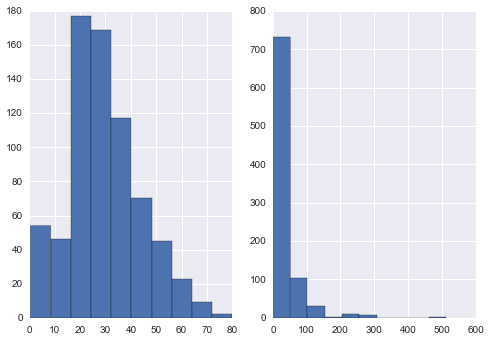
\includegraphics[width=50mm]{figures/train-age-fare.png}
}
\subfloat[test data]{
  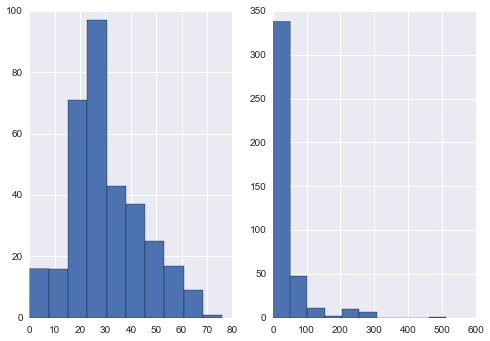
\includegraphics[width=50mm]{figures/test-age-fare.png}
}
\caption{Age (left) and fare (right) distributions}
\end{figure}

A couple of features in the dataset were ignored, namely \verb+Ticket+ and \verb+Cabin+. The difficulty of mapping these categorical values, which seem irrelevant, would likely outweigh any
benefits. Additionally, the values for \verb+Cabin+ were largely missing.

Following \href{https://www.kaggle.com/c/titanic/details/getting-started-with-python-ii}{the Kaggle article}, we constructed two new features from the dataset:
\verb+FamilySize+, obtained simply by adding together the number of siblings, spouses, parents and children aboard, and \verb+Age*Class+, obtained by multiplying age by the passenger's
socioeconomic status (1 for upper class, 2 for middle class, 3 for lower class), since both older and lower class passengers had a lower likelihood of survival.

At each decision step, we test the usefulness of a combination of features with a 10 fold cross-validation technique, which uses the code from Michael Wilber's lecture working with the \verb+cross_validation+
module in \verb+scikit-learn+ as a starting point.
Using \verb+FamilySize+ and \verb+Age*Class+ in place of \verb+Age+ both produced higher cross-validation scores.

We also experimented with pulling out the titles of each passenger's name and categorizing them in different ways. The first strategy was a binary approach with only pedestrian and non-pedestrian titles,
while the second strategy used 5 title types: pedestrian, honorary, academic, military, or religious. The latter approach resulted in higher cross-validation scores, though neither approach seemed to affect the Kaggle test results.
For reference, the attached code makes use of the second strategy, defined in \verb+get_title_type()+.

After running our solution on the test dataset, we submitted the results to Kaggle and received a score of 0.75598 as shown in Figure 2. For future improvements, experimenting with another model,
such as a random forest classifier, is recommended.
\begin{figure}
\centering
  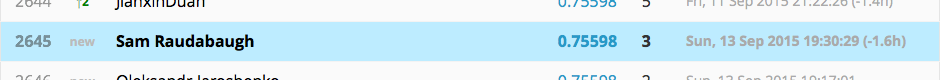
\includegraphics[width=150mm]{figures/kaggle-titanic.png}
\caption{Kaggle result for Titanic challenge}
\end{figure}
\newpage
\noindent{{\large Written 1. Variance of a sum}}
\\\\
Show var[X+Y] = var[X] + var[Y] + 2cov[X,Y].
\\\\
$var[X+Y] = cov[X+Y, X+Y]$
\\\\
By definition of covariance:
\\
$var[X+Y] = E[(X+Y)(X+Y)] - E[X+Y]E[X+Y]$
\\\\
$var[X+Y] = E[(X^2+2XY+Y^2]-(E[X]+E[Y])(E[X]+E[Y])$
\\\\
$var[X+Y] = E[X^2]-E[X]E[X] + E[Y^2]-E[Y]E[Y] + E[XY]-E[X]E[Y] + E[XY]-E[X]E[Y]$
\\\\
$var[X+Y] = cov[X,X] + cov[Y,Y] + cov[X,Y] + cov[X,Y]$
\\\\
$var[X+Y] = var[X] + var[Y] + 2cov[X,Y]$
\\\\
\noindent{{\large Written 2. Bayes rule for medical diagnosis}}
\\\\
Let $D$ refer to the event that you have the disease, and $TP$ refer to the event that you tested positive. Then:
\\\\
$P(D|TP) = \frac{P(D)P(TP|D)}{P(TP)}$
\\\\
Given $P(D) = 0.0001$ and $P(TP|D) = 0.99$, we only need to derive $P(TP)$.
\\\\
$P(TP) = P(TP|D)P(D)+P(TP|D')P(D')$
\\\\
Finally, with $P(TP|D') = 0.01$ and $P(D') = 0.9999$:
\\\\
$P(D|TP) = \frac{P(D)P(TP|D)}{P(TP|D)P(D)+P(TP|D')P(D')} = \frac{0.0001*0.99}{0.99*0.0001+0.01*0.9999} = 0.0098$
\newpage
\noindent{{\large Written 3a. Derivative of sigmoid function}}
\\\\
Given $\sigma(a) = \frac{1}{1+e^{-a}} = (1+e^{-a})^{-1}$
\\\\
$\frac{d\sigma(a)}{da} = -(1+e^{-a})^{-2}*-e^{-a}$
\\\\
$\frac{d\sigma(a)}{da} = \frac{e^{-a}}{(1+e^{-a})^2}$
\\\\
$\frac{d\sigma(a)}{da} = \frac{1}{1+e^{-a}}\left(\frac{e^{-a}}{1+e^{-a}}\right)$
\\\\
$\frac{d\sigma(a)}{da} = \frac{1}{1+e^{-a}}\left(\frac{1+e^{-a}}{1+e^{-a}} - \frac{1}{1+e^{-a}}\right)$
\\\\
$\frac{d\sigma(a)}{da} = \sigma(a)\left(1-\sigma(a)\right)$
\newpage
\noindent{{\large Written 3b. Gradient of log likelihood}}
\\\\
Given $l(\beta)=\sum_{i=1}^N\{y_ilogp(x_i;\beta)+(1-y_i)log(1-p(x_i;\beta))\}$
\\\\
$\frac{\delta l(\beta)}{\delta\beta}=\sum_{i=1}^N\frac{\delta}{\delta\beta}y_ilogp(x_i;\beta)+\sum_{i=1}^N\frac{\delta}{\delta\beta}(1-y_i)log(1-p(x_i;\beta))$
\\\\
Derive individual $\frac{\delta}{\delta\beta}$ terms:
\\\\
$\frac{\delta}{\delta\beta}y_ilogp(x_i;\beta)=y_i\cdot\frac{1}{p(x_i;\beta)}\cdot\frac{\delta}{\delta\beta}p(x_i;\beta)$
\\\\
$\frac{\delta}{\delta\beta}y_ilogp(x_i;\beta)=x_iy_i\cdot\frac{1}{p(x_i;\beta)}\cdot p(x_i;\beta)(1-p(x_i;\beta))=x_iy_i(1-p(x_i;\beta))$
\\\\
and:
\\\\
$\frac{\delta}{\delta\beta}(1-y_i)log(1-p(x_i;\beta))=(1-y_i)\frac{1}{1-p(x_i;\beta)}\cdot\frac{\delta}{\delta\beta}(1-p(x_i;\beta))$
\\\\
$\frac{\delta}{\delta\beta}(1-y_i)log(1-p(x_i;\beta))=\frac{1-y_i}{1-p(x_i;\beta)}\cdot-x_ip(x_i;\beta)(1-p(x_i;\beta))$
\\\\
$\frac{\delta}{\delta\beta}(1-y_i)log(1-p(x_i;\beta))=-x_i(1-y_i)p(x_i;\beta)$
\\\\
Plugging the terms into the original gradient, we simplify to the desired form:
\\\\
$\frac{\delta l(\beta)}{\delta\beta}=\sum_{i=1}^Nx_iy_i(1-p(x_i;\beta))-x_i(1-y_i)p(x_i;\beta)$
\\\\
$\frac{\delta l(\beta)}{\delta\beta}=\sum_{i=1}^Nx_i(y_i-y_ip(x_i;\beta)-(1-y_i)p(x_i;\beta))=\sum_{i=1}^Nx_i(y_i-p(x_i;\beta))$
\newpage
\noindent{{\large Written 3c. Proof that log likelihood Hessian is positive definite}}
\\\\
In order to prove that $X^TWX$ is positive definite, we must show that the scalar $v^TX^TWXv > 0$ for every $v$, which is any non-zero column vector of real numbers.
\\\\
Because $W$ is a diagonal matrix of non-negative real values $w_i$, we can absorb $W$ into $X$ and refactor $X^TWX$ into the following form:
\\\\
$X^TWX = Q^TQ$
\\\\
where each element of $Q$ is equal to the element at the same $i^{th}$ row and $j^{th}$ column in $X$, multiplied by $\sqrt{w_i}$.
\\\\
Plugging this new form into the expression $v^TX^TWXv$, we find that the expression can be represented as the inner product of $Qv$:
\\\\
$v^TX^TWXv = v^TQ^TQv = (Qv)^TQv = ||Qv||$
\\\\
which is a scalar representing the magnitude of a vector in Euclidian space, therefore it cannot be negative. Assuming nondegeneracy in the data (no duplicate inputs $x_i$), it also cannot be 0.
Therefore:
\\\\
$||Qv|| = v^TX^TWXv > 0$
\end{document}
